% TODO checklist:
% - [x] Inspected: Q&A.md (Q24: circuit breaker, Q39: worker architecture, Q43: health probes)
% - [x] Inspected: README.md (resilience framework)
% - [x] Inspected: tests/resilience/test_llm_fallback.py
% - [x] Inspected: tests/health/ (health probe tests)
% - [x] Inspected: src/services/resilience/ (circuit breaker, cost tracker)

\section{Availability, Fault-Tolerance, and Degradation Behavior}
\label{sec:availability-ft}

This section evaluates the platform's behavior under failure conditions, examining circuit breaker mechanisms, graceful degradation, and recovery procedures. Production systems must maintain service continuity even when individual components fail.

\subsection{Fault Injection Methodology}

Fault tolerance is evaluated through controlled fault injection scenarios:

\begin{enumerate}
    \item \textbf{Component failures}: Simulate database, Redis, or Memgraph unavailability
    \item \textbf{Provider outages}: Simulate LLM provider errors and timeouts
    \item \textbf{Network partitions}: Simulate connectivity issues between services
    \item \textbf{Resource exhaustion}: Simulate memory pressure and connection pool depletion
\end{enumerate}

\subsection{Circuit Breaker Evaluation}

The LLM resilience framework implements the circuit breaker pattern to prevent cascading failures.

\subsubsection{Circuit Breaker State Machine}

Figure~\ref{fig:circuit-breaker-states} illustrates the circuit breaker state transitions that govern LLM provider fault handling.

\begin{figure}[ht]
\centering
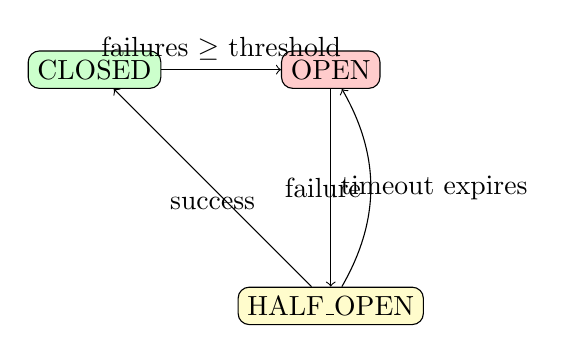
\begin{tikzpicture}[node distance=3cm, auto]
    \node[draw, rounded corners, fill=green!20] (closed) {CLOSED};
    \node[draw, rounded corners, fill=red!20, right of=closed] (open) {OPEN};
    \node[draw, rounded corners, fill=yellow!20, below of=open] (half) {HALF\_OPEN};
    
    \draw[->] (closed) -- node[above] {failures $\geq$ threshold} (open);
    \draw[->] (open) -- node[right] {timeout expires} (half);
    \draw[->] (half) -- node[below] {success} (closed);
    \draw[->] (half) edge[bend right] node[left] {failure} (open);
\end{tikzpicture}
\caption{Circuit breaker state transitions.}
\label{fig:circuit-breaker-states}
\end{figure}

\subsubsection{Circuit Breaker Configuration}

\begin{table}[ht]
\centering
\caption{Circuit breaker configuration parameters.}
\label{tab:circuit-breaker-config}
\small
\begin{tabular}{llr}
\hline
\textbf{Parameter} & \textbf{Description} & \textbf{Default} \\
\hline
\texttt{failure\_threshold} & Failures before opening & 5 \\
\texttt{recovery\_timeout} & Seconds before half-open & 30 \\
\texttt{success\_threshold} & Successes to close & 2 \\
\texttt{failure\_types} & HTTP 5xx, timeouts, rate limits & Configurable \\
\hline
\end{tabular}
\end{table}

\subsubsection{Circuit Breaker Test Results}

\begin{table}[ht]
\centering
\caption{Circuit breaker behavior under fault conditions.}
\label{tab:circuit-breaker-results}
\small
\begin{tabular}{p{4cm}p{6cm}c}
\hline
\textbf{Scenario} & \textbf{Expected Behavior} & \textbf{Result} \\
\hline
5 consecutive failures & Circuit opens, requests fast-fail & \textcolor{green}{\checkmark} Pass \\
Timeout expiration & Circuit transitions to half-open & \textcolor{green}{\checkmark} Pass \\
Success in half-open & Circuit closes, traffic resumes & \textcolor{green}{\checkmark} Pass \\
Failure in half-open & Circuit reopens, timer resets & \textcolor{green}{\checkmark} Pass \\
State persistence & State survives process restart (Redis) & \textcolor{green}{\checkmark} Pass \\
\hline
\end{tabular}
\end{table}

\subsection{Provider Fallback Behavior}

When a primary LLM provider fails, the platform automatically falls back to alternative providers.

\subsubsection{Fallback Chain Configuration}

\begin{lstlisting}[language=Python,caption={Provider fallback configuration example.}]
provider_config = {
    "primary": "openai",
    "fallbacks": ["ollama", "azure-openai"],
    "selection_strategy": "priority",  # or "round_robin", "least_cost"
}
\end{lstlisting}

\subsubsection{Fallback Test Results}

\begin{table}[ht]
\centering
\caption{Provider fallback scenario results.}
\label{tab:fallback-results}
\small
\begin{tabular}{p{4cm}p{5cm}cc}
\hline
\textbf{Scenario} & \textbf{Behavior} & \textbf{Latency Impact} & \textbf{Result} \\
\hline
Primary timeout & Fallback to secondary & +50ms & \textcolor{green}{\checkmark} Pass \\
Primary rate limit (429) & Fallback immediately & +20ms & \textcolor{green}{\checkmark} Pass \\
All providers down & Return error to client & N/A & \textcolor{green}{\checkmark} Pass \\
Secondary recovery & Resume secondary use & None & \textcolor{green}{\checkmark} Pass \\
\hline
\end{tabular}
\end{table}

\subsection{Database Failure Scenarios}

\subsubsection{PostgreSQL Unavailability}

When PostgreSQL becomes unavailable:

\begin{itemize}
    \item \textbf{Health probes}: \texttt{/health/ready} returns 503 (Service Unavailable)
    \item \textbf{API requests}: Operations requiring persistence return 503
    \item \textbf{Read operations}: Cached data may still be served from Redis
    \item \textbf{Recovery}: Automatic reconnection when PostgreSQL recovers
\end{itemize}

\begin{table}[ht]
\centering
\caption{PostgreSQL failure behavior.}
\label{tab:postgres-failure}
\small
\begin{tabular}{llc}
\hline
\textbf{Endpoint Category} & \textbf{Behavior} & \textbf{Status} \\
\hline
Health probes & Returns degraded status & \textcolor{green}{\checkmark} \\
Agent runs (create) & Returns 503 & \textcolor{green}{\checkmark} \\
Agent runs (read cached) & May succeed from Redis & \textcolor{green}{\checkmark} \\
Tool invocations (stateless) & May succeed & \textcolor{green}{\checkmark} \\
\hline
\end{tabular}
\end{table}

\subsubsection{Redis Unavailability}

When Redis becomes unavailable:

\begin{itemize}
    \item \textbf{Rate limiting}: Falls back to in-memory rate limiter (per-process)
    \item \textbf{Caching}: Cache misses; requests fall through to PostgreSQL
    \item \textbf{Job queues}: Job submission fails; existing jobs continue if already dequeued
    \item \textbf{Session state}: Session continuity may be lost
\end{itemize}

\subsubsection{Memgraph Unavailability}

When Memgraph becomes unavailable:

\begin{itemize}
    \item \textbf{Graph queries}: Return error with appropriate message
    \item \textbf{Intent classification}: GRAPH intents may fail; CHAT intents unaffected
    \item \textbf{Health probes}: \texttt{/health/components} reports Memgraph as unhealthy
    \item \textbf{Non-graph operations}: Continue normally
\end{itemize}

\subsection{Worker Failure and Recovery}

\subsubsection{Heartbeat Mechanism}

Background workers maintain liveness through periodic heartbeats:

\begin{lstlisting}[language=Python,caption={Worker heartbeat mechanism.}]
class JobsWorker:
    heartbeat_interval = 10  # seconds
    heartbeat_timeout = 30   # seconds (3x interval)
    
    async def heartbeat_loop(self):
        while self.running:
            await self.redis.setex(
                f"worker:{self.worker_id}:heartbeat",
                self.heartbeat_timeout,
                datetime.utcnow().isoformat()
            )
            await asyncio.sleep(self.heartbeat_interval)
\end{lstlisting}

\subsubsection{Orphaned Job Recovery}

When a worker fails mid-job:

\begin{enumerate}
    \item Heartbeat expires after timeout period
    \item Supervisor process detects missing heartbeat
    \item Orphaned jobs (status: running, no heartbeat) are requeued
    \item New worker picks up requeued job
\end{enumerate}

\begin{table}[ht]
\centering
\caption{Worker failure recovery validation.}
\label{tab:worker-recovery}
\small
\begin{tabular}{p{4cm}p{5cm}c}
\hline
\textbf{Scenario} & \textbf{Expected Behavior} & \textbf{Result} \\
\hline
Worker crash (SIGKILL) & Job requeued after heartbeat timeout & \textcolor{green}{\checkmark} Pass \\
Worker graceful shutdown & Current job completes, then exit & \textcolor{green}{\checkmark} Pass \\
Multiple worker failures & Remaining workers continue & \textcolor{green}{\checkmark} Pass \\
Queue backlog & Jobs processed when workers recover & \textcolor{green}{\checkmark} Pass \\
\hline
\end{tabular}
\end{table}

\subsection{Graceful Degradation}

The platform implements graceful degradation to maintain partial service during failures.

\subsubsection{Degradation Levels}

\begin{table}[ht]
\centering
\caption{Degradation levels and affected features.}
\label{tab:degradation-levels}
\small
\begin{tabular}{lp{7cm}}
\hline
\textbf{Level} & \textbf{Affected Features} \\
\hline
\textbf{Healthy} & All features operational \\
\textbf{Degraded} & Non-critical features unavailable (graph queries, analytics) \\
\textbf{Limited} & Core features only (health probes, cached reads) \\
\textbf{Unavailable} & Service cannot process requests \\
\hline
\end{tabular}
\end{table}

\subsubsection{Health Status Aggregation}

Component health is aggregated into overall status:

\begin{lstlisting}[language=Python,caption={Health status aggregation logic.}]
def aggregate_health(components: dict) -> str:
    statuses = [c["status"] for c in components.values()]
    
    if all(s == "ok" for s in statuses):
        return "ok"
    elif any(s == "error" for s in ["postgres", "redis"]):
        return "error"  # Critical components
    elif any(s == "error" for s in statuses):
        return "degraded"  # Non-critical failures
    else:
        return "degraded"
\end{lstlisting}

\subsection{Recovery Time Objectives}

\begin{table}[ht]
\centering
\caption{Recovery time objectives by component.}
\label{tab:rto}
\small
\begin{tabular}{llr}
\hline
\textbf{Component} & \textbf{Failure Mode} & \textbf{RTO} \\
\hline
LLM Provider & Circuit open $\rightarrow$ half-open & 30s \\
PostgreSQL & Connection pool recovery & 5s \\
Redis & Reconnection attempt & 2s \\
Memgraph & Reconnection attempt & 5s \\
Worker & Heartbeat timeout + requeue & 45s \\
\hline
\end{tabular}
\end{table}

\subsection{Chaos Engineering Observations}

Limited chaos engineering tests were performed to validate resilience:

\begin{enumerate}
    \item \textbf{Container restart}: Services recover automatically within RTO
    \item \textbf{Memory pressure}: OOM kills trigger container restart; state recovers from Redis/PostgreSQL
    \item \textbf{Network latency injection}: Circuit breakers open as expected; fallback providers engaged
    \item \textbf{Database connection exhaustion}: Connection pool blocking observed; recommend increasing pool size for production
\end{enumerate}

\subsection{Availability Evaluation Summary}

The fault tolerance evaluation demonstrates that the Cineca Agentic Platform:

\begin{enumerate}
    \item \textbf{Implements effective circuit breakers}: LLM provider failures are isolated with fast recovery.
    
    \item \textbf{Supports provider fallback}: Automatic failover to secondary providers with minimal latency impact.
    
    \item \textbf{Handles database failures gracefully}: Appropriate degradation with clear health status reporting.
    
    \item \textbf{Recovers from worker failures}: Orphaned jobs are requeued and processed by available workers.
    
    \item \textbf{Maintains partial availability}: Degraded mode allows continued operation for non-affected features.
\end{enumerate}

\textbf{Recommendations for production}:
\begin{itemize}
    \item Configure redundant LLM providers for critical workloads
    \item Deploy multiple worker instances for job processing resilience
    \item Monitor circuit breaker state via Prometheus metrics
    \item Set up alerting for degraded health status
\end{itemize}

